\documentclass[../thesis.tex]{subfiles}

\begin{document}
\chapter{System Overview}


\section{Concept}

The solar panel generates electricity and feed it into the converter after being measured by the current and voltage sensor. The converter converts the electricity from a higher voltage to a desired votlage, which can be measured again by the sensor and used to charge the battery. The sensing data consist of input current and voltage, and output current and voltage, which are fed into the microcontroller. The microcontroller has a 4G cellular modem which enables communication with the surrounding 4G cellular base station, and the internet access is provided by the gateway at the base station. That means, the sensing data can be be sent from the microcontroller to the server  through 4G cellular network. Once the sensing data reaches the server, the data is processed, store into the database, and send to the client such as a web application. The concept is shown in the figure \ref{fig:concept1}.

\begin{figure}[!ht]
  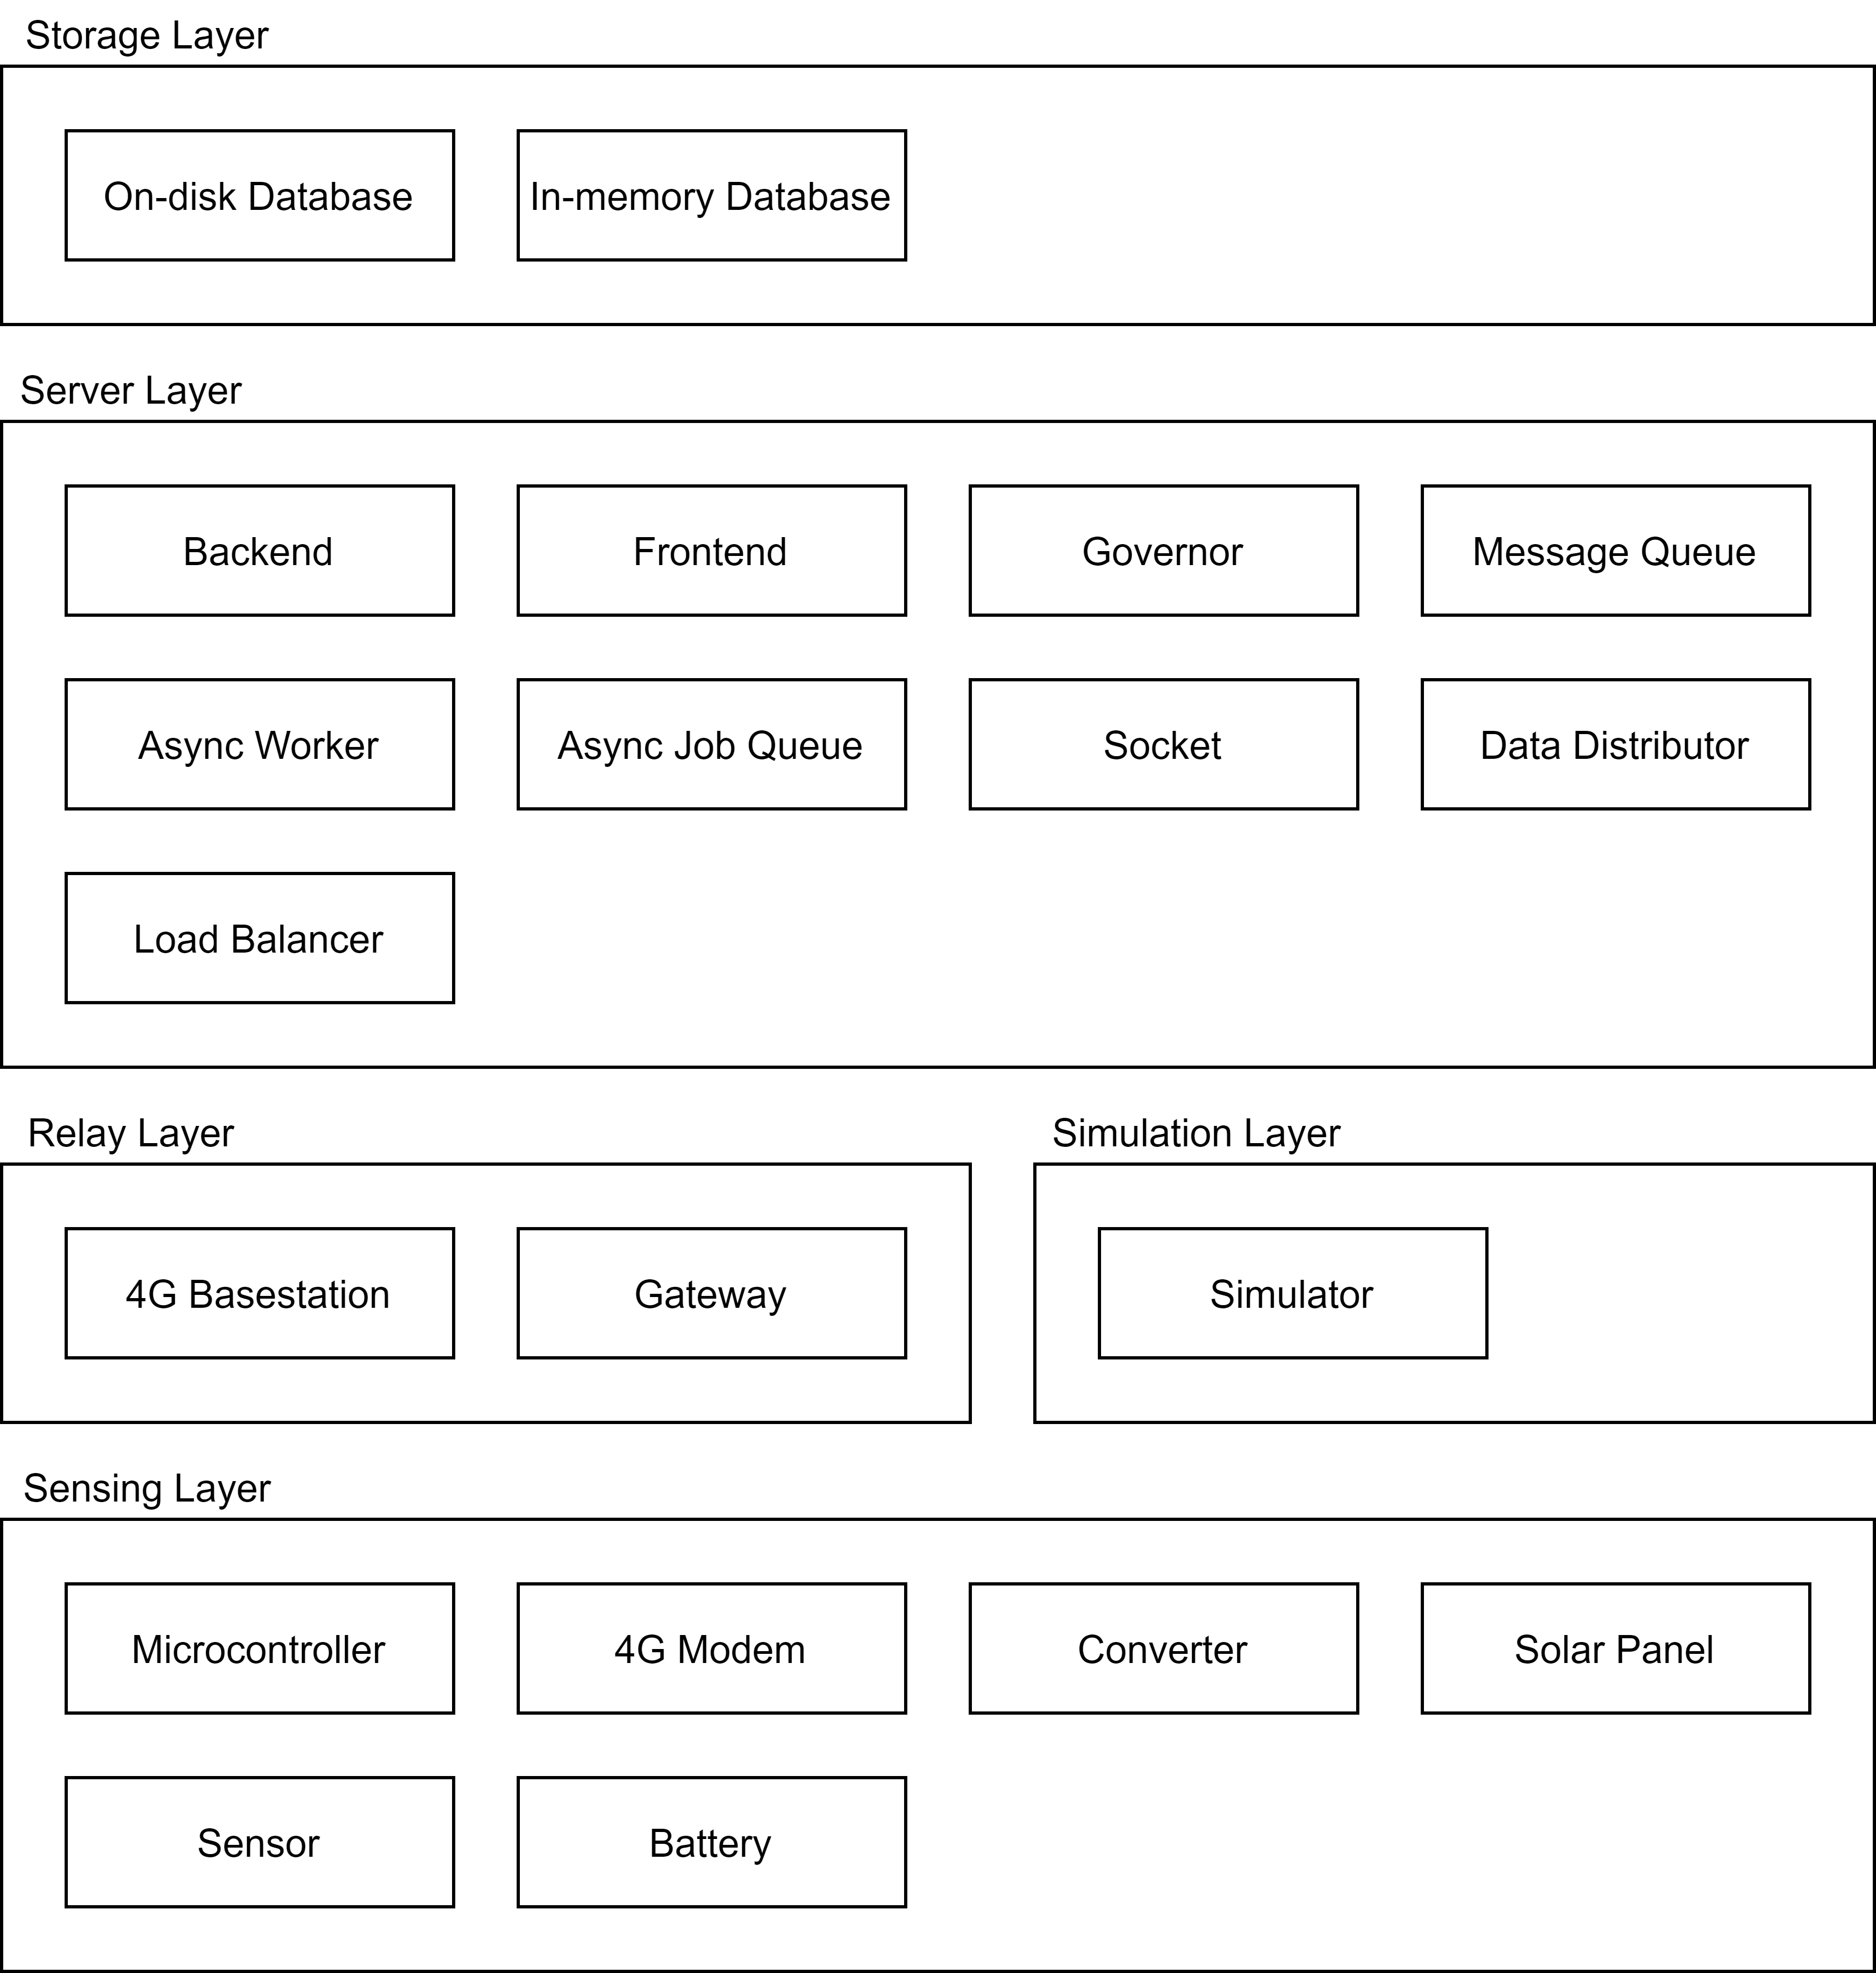
\includegraphics[width=\linewidth]{c3-concept-1.png}
  \caption{Concept of the proposed system.}
  \label{fig:concept1}
\end{figure}


\section{Composition}

The systems is composed of 



\begin{figure}[!ht]
  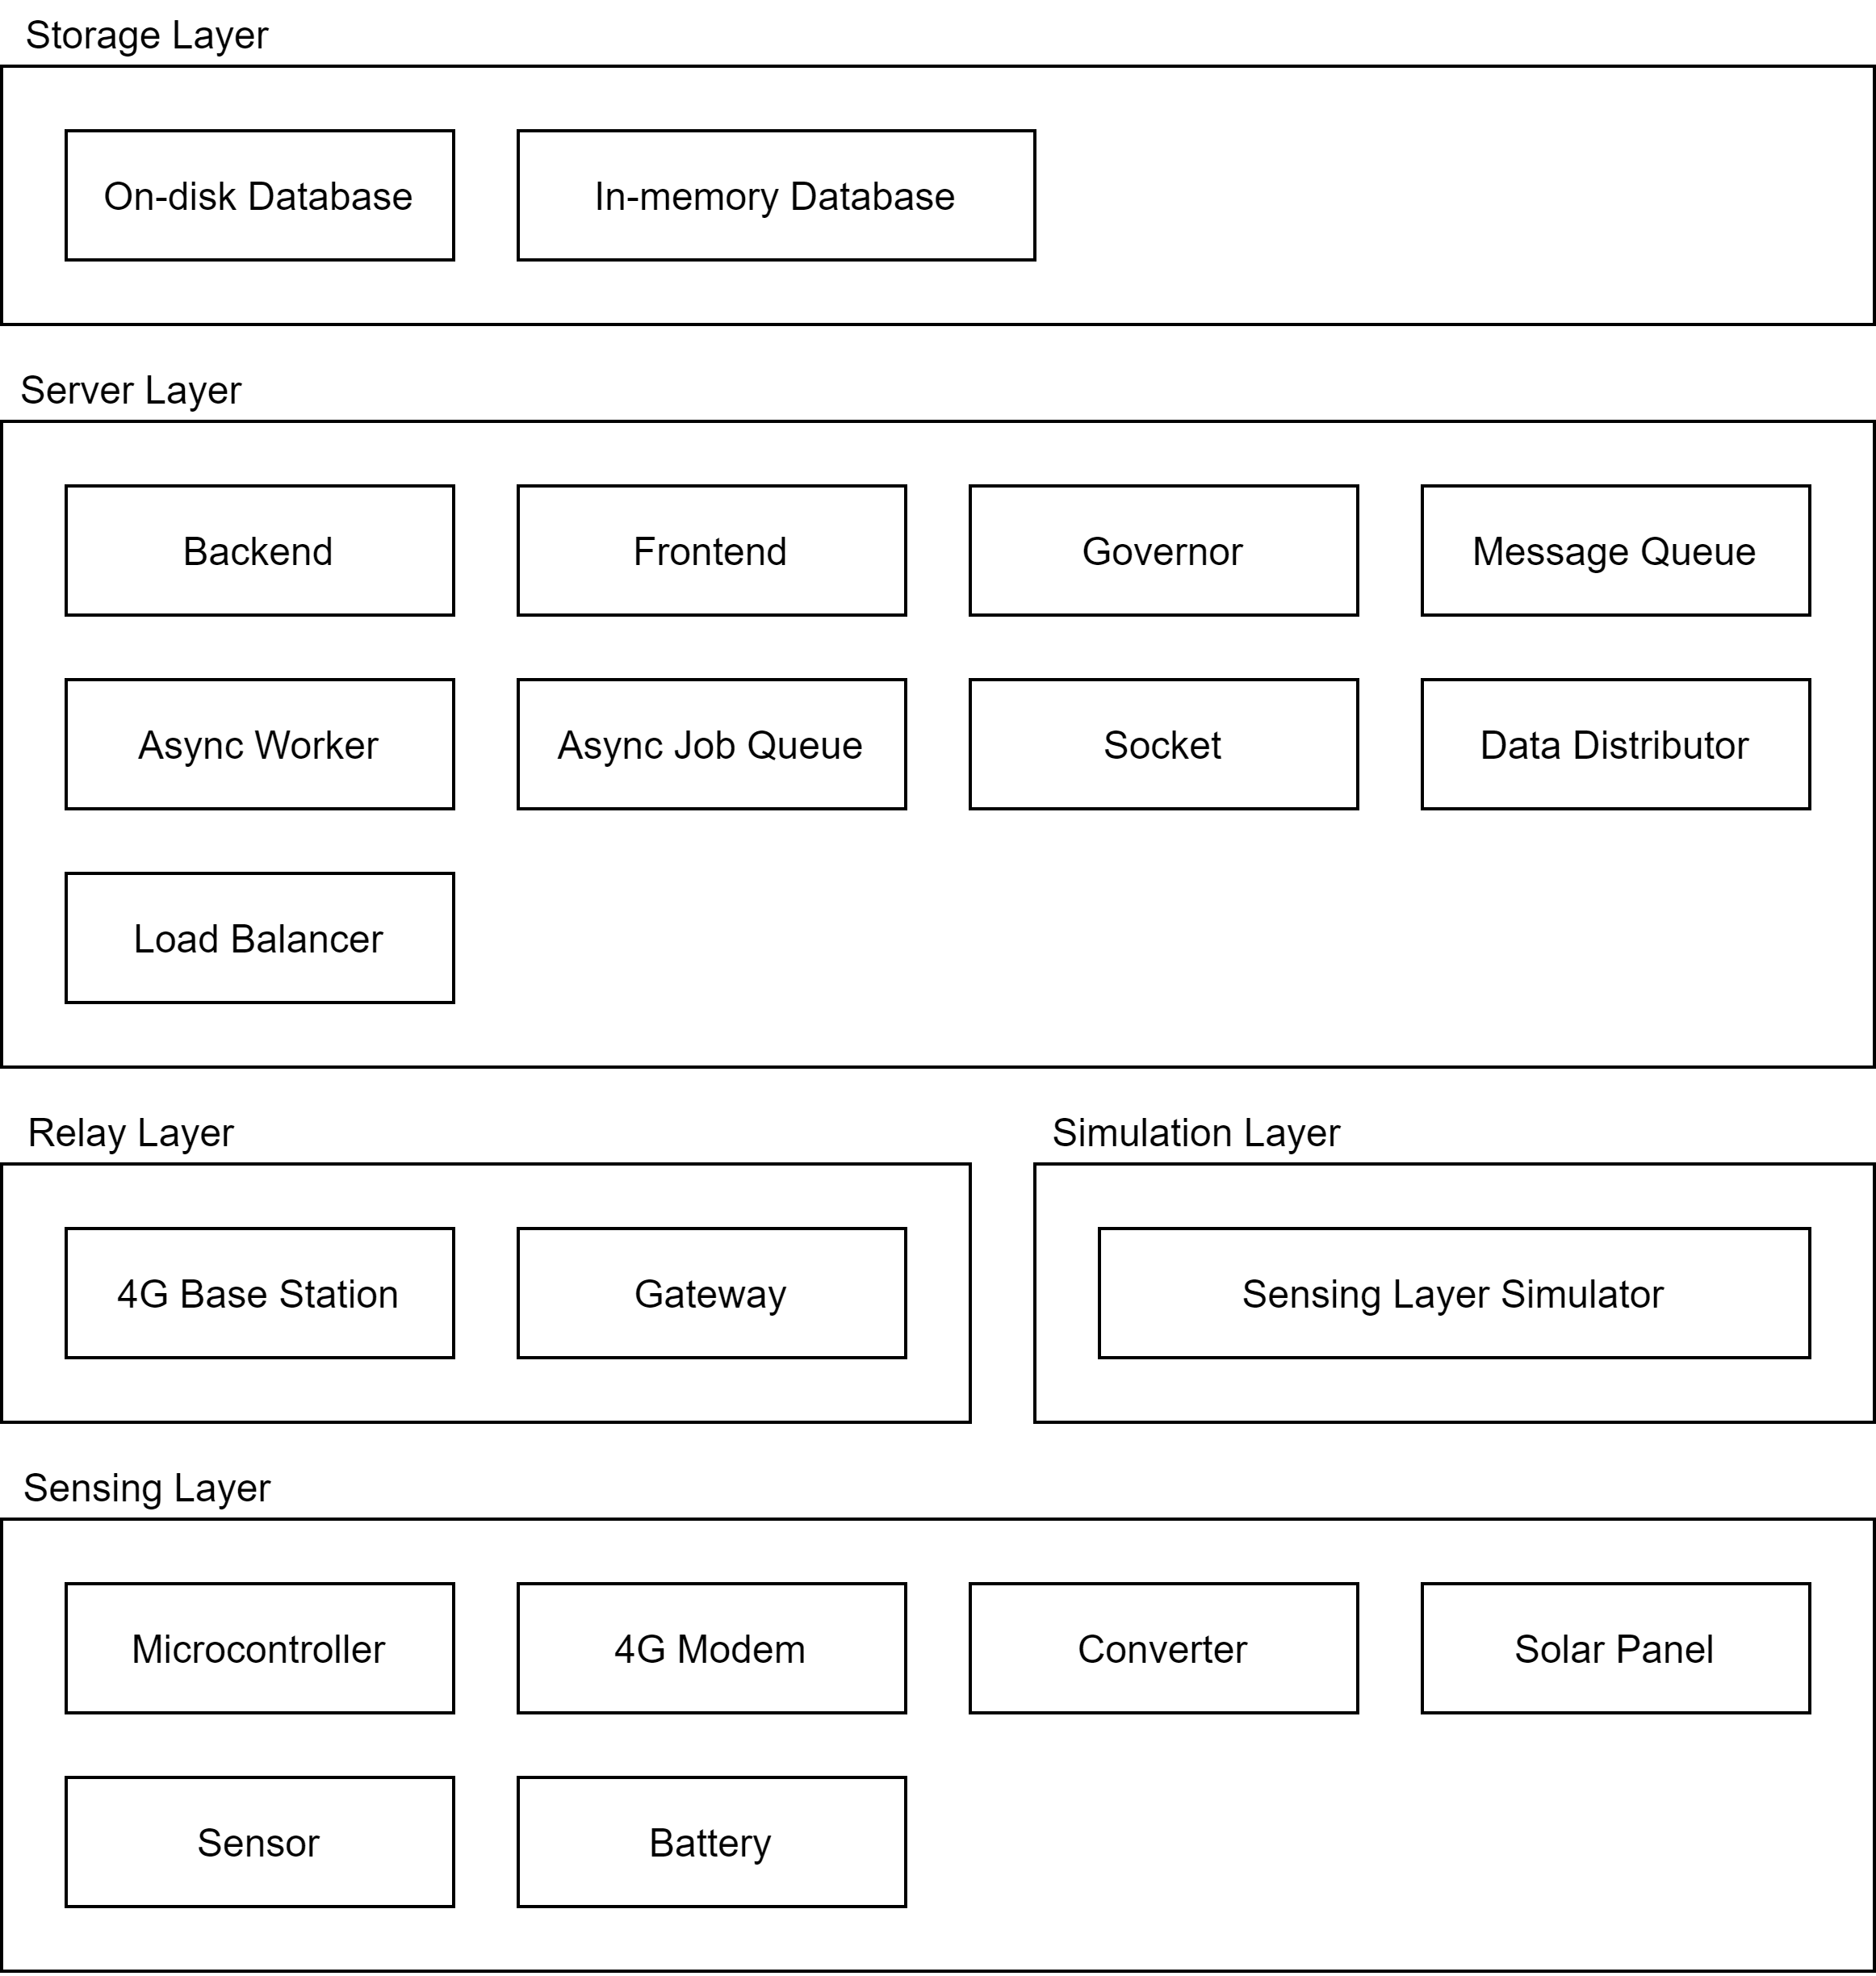
\includegraphics[width=\linewidth]{c3-concept-2.png}
  \caption{Layers and components of the proposed system.}
  \label{fig:concept2}
\end{figure}


\section{Hardware}

asdfsadfasdfasdfasdf

\section{Software}

asdfsadfasdfasdfasdf

\section{Cost estimate}

asdfsadfasdfasdfasdf

\end{document}